\documentclass[american,a4paper,12pt]{article}
\usepackage[T1]{fontenc} %for å bruke æøå
\usepackage[utf8]{inputenc}
\usepackage{graphicx} %for å inkludere grafikk
\usepackage{verbatim} %for å inkludere filer med tegn LaTeX ikke liker
\usepackage{mathpazo}
\usepackage{algorithm} % for algoritmene e.g paragraf 2.2 Gauss
\usepackage{algpseudocode} % lager pseudokode til algoritmene
\usepackage{amsmath}
\usepackage{caption}
\usepackage{multicol}
\usepackage{siunitx}
\usepackage{float}
\usepackage{subcaption}
\usepackage{hyperref}
\hypersetup{
    colorlinks=true,
    linkcolor=black,
    filecolor=magenta,
    urlcolor=blue,
    citecolor=blue
    pdftitle={Project 1: Computational Physics - FYS3150},
    pdfpagemode=FullScreen
}



\renewcommand{\vec}[1]{\mathbf{#1}} %ny definisjon av \vec så det blir bold face i stedet for vector-pil.


\captionsetup[table]{skip=10pt}
\bibliographystyle{plain}

\title{Project 1: Computational Physics - FYS3150}
\author{Fredrik Hoftun \& Mikkel Metzsch Jensen}
\date{September 09, 2020}
\begin{document}
\maketitle

\tableofcontents


\begin{abstract}
  The goal of this project were to... \\
  What did we do? \\
  What did we find? \\
\end{abstract}

\section{Introduction}
  In this project we will investegate different numerical approaches for the solving of the one-dimensional Poisson equation with Dirichlet boundary conditions. This is a problem that is used in many different scientiffic applications. It is used to describe electrostatic and megnetostatic phenonema in a quantitative maner. It is also helps to understand diffusion and propagation problems. The solution is generally used in a wide range of fields such as engineering, physics, mathematics, biology, chemistry, etc. \cite{poisson_paper}. In this project we have used a second derivative approximation in order to rewrite the problem as a set of linear equations. We have written three different algorithms: A general and a specialiazed algorithm using gaussian elimination and then LU demposition. Theese are described individually in the method sections along with a calculation of the number of floating point operation for each of them. Since we know the analytical solution for our problem we have compaired relative error for different choices of stepsize $h$ in the algorithm. We have also compaired of the CPU time of theese computationg. We found a significant difference in both precesion (due to round of erros) and CPU time, which are presented in the results section.

  \begin{enumerate}
    \item Motivate the reader
    \item What have I done
    \item The structure of the report
    \item conlusion?
  \end{enumerate}





\section{Method}
  \subsection{Defining the problem}
    We are going to solve the one-dimensional Poisson equation with Dirichlet boundary conditions given as the following:
    \begin{align*}
      u''(x) = f(x), \quad x \in (0,1), \quad u(0) = u(1) = 0
    \end{align*}
    In our case we will use the function:
    \begin{align*}
      f(x) = 100e^{-10x}
    \end{align*}
    Note that the algorithms for solving the problem will not be depedent on this specefic choice of f(x). The reason why we stick to this function is for the praticality of having the following analytical solution for f(x):
    \begin{align*}
      u(x) = 1 - (1 - e^{-10})x - e^{-10x}
    \end{align*}
    We can ensure that this is a valid Sslution by inserting it into the Poission equation. First we calculate double derivative of u(x):
    \begin{align*}
      u'(x) = -(1 - e^{-10}) + 10e^{-10x}, \quad u''(x) = -100e^{-10x}
    \end{align*}
    We now see that the solution satisfies the Poisson equation:
    \begin{align*}
      -u''(x) = 100e^{-10x} = f(x)
    \end{align*}
    We can therefore use this analytical solution to evaluate the precision of the numerical solutions for different choices of step length $h$.
  \subsection{Rewritting the problem as a set of linear equations}
    In order to solve the Poisson equation numerically we discretize u as $v_i$ with $n + 2$ grid points $x_i = ih$ for $i = 0, 1, \hdots, n + 1$. To clarify we have $x_0 = 0$, $x_{n+1} = 1$ which are spaced with step length $h = 1/(n + 1)$. The boundary conditions is then $v_0 = v_{n+1} = 0$. We use the following second derivative approximation
    \begin{center}
      $-u''(x_i) \approx -\frac{v_{i+1} + 2v_i - v_{i+1}}{h^2} =  f(x_i)$ \quad for $i = 1, \hdots, n$
    \end{center}
    $\Longleftrightarrow$
    \begin{align*}
      -v_{i-1} + 2v_i - v_{i+1} = h^2f(x_i)
    \end{align*}
    Notice that we cannot calculate the second derivative approximation at the end points $i = 0$ and $i = n + 1$ since we need avaliable points $v_{\pm 1}$ for the calculation. We define the colum vector $\vec{v} = [v_1, v_2, \hdots, v_n]$ and try to setup the equation for every step $i = 1, \hdots, n$. As we do this we see a usefull pattern appearing
    \begin{align*}
          \begin{bmatrix}
            2 & -1 & 0 & \cdots & 0
          \end{bmatrix}
          \begin{bmatrix}
            v_1 \\
            \vdots \\
            v_n
          \end{bmatrix}
    = h^2f(x_1)
    \end{align*}
    \begin{align*}
          \begin{bmatrix}
            2 & -1 & 0 & \cdots & \cdots & 0 \\
            -1 & 2 & -1 & 0 & \cdots & \cdots
          \end{bmatrix}
          \begin{bmatrix}
            v_1 \\
            \vdots \\
            v_n
          \end{bmatrix}
    = h^2
          \begin{bmatrix}
            f(x_1) \\
            f(x_2)
          \end{bmatrix}
    \end{align*}
    \begin{align*}
      \vdots
    \end{align*}
    \begin{align*}
          \begin{bmatrix}
            2 & -1 & 0 & \cdots & \cdots & 0 \\
            -1 & 2 & -1 & 0 & \cdots & \cdots \\
            0 & -1 & 2 & -1 & 0 & \cdots \\
            \cdots & \cdots & \cdots & \cdots & \cdots & \cdots \\
            0 & \cdots & & -1 & 2 & -1 \\
            0 & \cdots & & 0 & -1 & 2
          \end{bmatrix}
          \begin{bmatrix}
            v_1 \\
            \vdots \\
            v_n
          \end{bmatrix}
    = h^2
          \begin{bmatrix}
            f(x_1) \\
            f(x_2) \\
            \vdots \\
            f_n
          \end{bmatrix}
    \end{align*}
    \\ From this we see that we can write the problem as a linear set of equation:
    \begin{align*}
      \vec{A}\vec{v} = \vec{g}
    \end{align*}
    With the following definitions:\\
    \begin{align*}
      \vec{A} =
      \begin{bmatrix}
        2 & -1 & 0 & \cdots & \cdots & 0 \\
        -1 & 2 & -1 & 0 & \cdots & \cdots \\
        0 & -1 & 2 & -1 & 0 & \cdots \\
        \cdots & \cdots & \cdots & \cdots & \cdots & \cdots \\
        0 & \cdots & & -1 & 2 & -1 \\
        0 & \cdots & & 0 & -1 & 2
      \end{bmatrix}
      \quad, \vec{v} =
      \begin{bmatrix}
        v_1 \\
        v_2 \\
        \vdots \\
        v_n
      \end{bmatrix}
      \quad, \vec{\tilde{g}} = h^2
      \begin{bmatrix}
        f(x_1) \\
        f(x_2) \\
        \vdots \\
        f_n
      \end{bmatrix}
    \end{align*}
\subsection{General solution using Gausian elimination}
We can solve our set of linear equations using Gaussian elimination on the matrix $\vec{A}\vec{v} = \vec{g}$. In the beginning we assume a more generilazed matrix $\vec(A)$ as:
\begin{align*}
  A =
  \begin{bmatrix}
    b_1 & c_1 & 0 & \cdots & \cdots & 0 \\
    a_1 & b_2 & c_2 & 0 & \cdots & \cdots \\
    0 & a_2 & b_3 & c_3 & 0 & \cdots \\
    \cdots & \cdots & \cdots & \cdots & \cdots & \cdots \\
    0 & \cdots & & a_{n-2} & b_{n-1} & c_{n-1} \\
    0 & \cdots & & 0 & a_{n-1} & b_n
  \end{bmatrix}
\end{align*}
\\ Here $a_i$ are the elements below the diagonal, $b_i$ are the elements on the diagonal and $c_i$ are the elements above the diagonal. In order to solve this we use first a forward substitution and then a backwards substitution \cite{linalg}. The implementation of this is showed in Algorithm 1:
\begin{algorithm}[H]
\caption{General algorithm}
\begin{algorithmic}[1] %fra algpseudocode
  \For {$i = 2, \dots, n$} \Comment{Forward substitution eliminating $a_i$}
    \State $b_i = b_i - c_{i-1}\cdot {a_i}/{{b}_{i-1}}$ \Comment{Update ${b}_i$}
    \State $g_i = g_i - {g}_{i-1}\cdot {a_i}/{{b}_{i-1}}$ \Comment{Update ${g}_i$}
  \EndFor
  \Statex
  \State $v_n = g_n/B_n;$ \Comment{Backward substitution obtaining $v_i$}
  \For {$i = n-1, \dots, 1$}
    \State $v_i = (g_i - c_i\cdot v_{i+1})/b_i$ % \frac{g_i - c_i\cdot v_{i+1}}{b_i}$
  \EndFor
\end{algorithmic}
\end{algorithm}
We can calculate the algorithms number of Floating Point Operations. In our forward substitution we have $2 \cdot 3$ operations for each loop which runs for a total of n-1 times. In the backward substitution we have a single leading operation and then 3 operations which loops for a total of n-1. The total number of operations is then
\begin{align*}
  (6 + 3)(n - 1) + 1 = 9n - 8
\end{align*}
For large n we can approximate this as 9n. 
\subsection{Simplified specific solution}
In this specific case we have $a = -1,\ b = 2,\ c = -1$ which means we can further simplify our matrix $\vec{A}$:
\begin{align*}
    \vec{A} =
    \begin{bmatrix}
    2 & -1 & 0 & \cdots & \cdots & 0 \\
    -1 & 2 & -1 & 0 & \cdots & \cdots \\
    0 & -1 & 2 & -1 & 0 & \cdots \\
    \cdots & \cdots & \cdots & \cdots & \cdots & \cdots \\
    0 & \cdots & & -1 & 2 & -1 \\
    0 & \cdots & & 0 & -1 & 2
    \end{bmatrix}
    \ \sim \
    \begin{bmatrix}
    2 & -1 & 0 & \cdots & \cdots & 0 \\
    0 & 3/2 & -1 & 0 & \cdots & \cdots \\
    0 & -1 & 2 & -1 & 0 & \cdots \\
    \cdots & \cdots & \cdots & \cdots & \cdots & \cdots \\
    0 & \cdots & & -1 & 2 & -1 \\
    0 & \cdots & & 0 & -1 & 2
    \end{bmatrix}
\end{align*}
\begin{align*}
    \quad \sim
    \begin{bmatrix}
    2 & -1 & 0 & \cdots & \cdots & 0 \\
    0 & 3/2 & -1 & 0 & \cdots & \cdots \\
    0 & 0 & 4/3 & -1 & 0 & \cdots \\
    \cdots & \cdots & \cdots & \cdots & \cdots & \cdots \\
    0 & \cdots & & -1 & 2 & -1 \\
    0 & \cdots & & 0 & -1 & 2
    \end{bmatrix}
    \ \sim \
    \begin{bmatrix}
    2 & -1 & 0 & \cdots & \cdots & 0 \\
    0 & 3/2 & -1 & 0 & \cdots & \cdots \\
    0 & 0 & 4/3 & -1 & 0 & \cdots \\
    \cdots & \cdots & \cdots & \cdots & \cdots & \cdots \\
    0 & \cdots & & 0 & i_n/{i_n-1} & -1 \\
    0 & \cdots & & 0 & 0 & {i_n+1}/i_n
    \end{bmatrix} \\
\end{align*}
Where we have called the last diagonal element $i_n$. We see that $b_i = \frac{i+1}{i}$, reducing the computation time. With our new $b_i$ we can create a new algorithm.
\begin{algorithm}
\caption{Special algorithm, where $a_i = -1,\ b_i = 2,\ c_i = -1$}
\begin{algorithmic}[1]
  \For {$i = 2, \dots, n$} \Comment{Forward substitution eliminating $a_i$}
    \State $b_i = {i+1}/i$ \Comment{Update ${b}_i$}
    \State $g_i = g_i + {g}_{i-1}/{{b}_{i-1}}$ \Comment{Update ${g}_i$}
  \EndFor

  \Statex
  \State $v_n = 0$ \Comment{Backward substitution obtaining $v_i$}
  \For {$i = n-1, \dots, 1$}
    \State $v_i = \frac{g_i + v_{i+1}}{b_i}$
  \EndFor
\end{algorithmic}
\end{algorithm}

Similarly to the general algorithm we can calculate total FLOPS:
\begin{center}
    $(2*2+2)(n-2)+1 = 6n-11$
\end{center}
Which for large $n$ is considerably less. If we take into a account that $b_i = \frac{i+1}{i}$ can be precalculated for all $i \in [1, \hdots, n]$ before hand, we get a total number of FP:
\begin{align*}
  (2 + 2)(n-2) = 4n - 8
\end{align*}
which for large n can be approximated to $4n$
\subsection{LU decomposition}
For the LU decomposition we ...\\
FLOPS $O(n^3)$ se \url{https://en.wikipedia.org/wiki/LU_decomposition}, søk etter "float"

\subsection{Comparing precision and error}


\subsection{Implementation}
We used \verb!C++! to implement our algorithms ... and we used Pythons library Matplotlib to plot our results.

\section{Results}
  GITHUB LINK HERE \\
  Max error:
  \begin{figure}[H]
  \begin{center}
    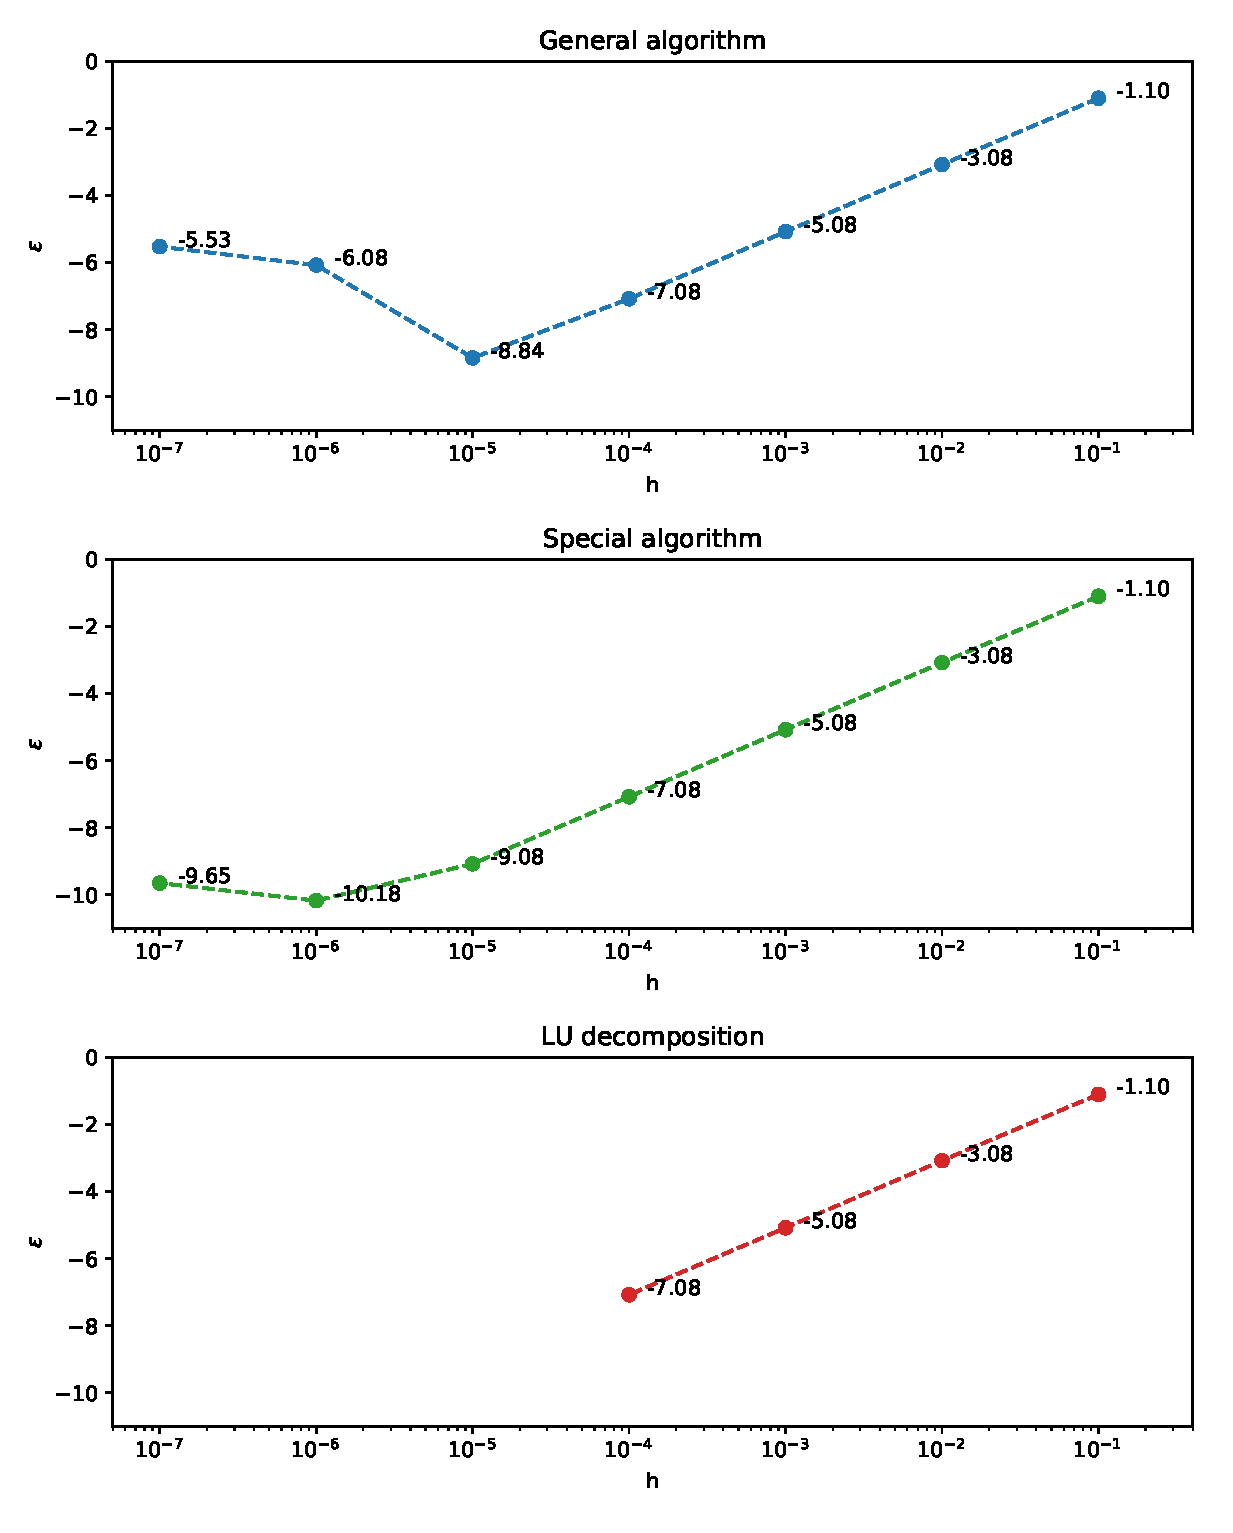
\includegraphics[width = \textwidth]{figures/max_err.eps} \\
    \caption{Log10 of the maximum error for each numerical solution compared to the analytical solution for different number of gridpoints n and different numerical methods.}
    \label{fig:max_err}
    \end{center}
  \end{figure}




  \begin{table}[H]
    \begin{center}
    \caption{CPU Time}
    \begin{tabular}{|c|c|c|c|} \hline
    \textbf{N} & \textbf{General algorithm: t [s]} & \textbf{Special algorithm: t [s]} & \textbf{LU Decomposition: t [s]} \\ \hline
    $10^1$ & $\num{3e-6}$     & $\num{3e-6}$    & $\num{9.81e-4}$ \\ \hline
    $10^2$ & $\num{4e-6}$     & $\num{4e-6}$    & $\num{1.96e-4}$ \\ \hline
    $10^3$ & $\num{3.8e-5}$   & $\num{3.7e-5}$  & $\num{1.02e-2}$ \\ \hline
    $10^4$ & $\num{3.41e-4}$  & $\num{3.54e-4}$ & $\num{2.45e0}$ \\ \hline
    $10^5$ & $\num{3.79e-3}$  & $\num{3.50e-3}$ & nan \\ \hline
    $10^6$ & $\num{3.57e-2}$  & $\num{3.24e-2}$ & nan \\ \hline
    $10^7$ & $\num{3.16e-1}$  & $\num{3.24e-1}$ & nan \\ \hline
    \end{tabular}
    \end{center}
    \label{tab:final_res}
  \end{table}

  Computer specs:
  \begin{center}
    CPU = 2.5 GHz Intel Core i5
  \end{center}


\subsection{General algorithm}

\subsection{Special algorithm}

\subsection{LU decomposition}

\section{Discussion}
Error analysis \\
\\
The computer should be able to make a maximum of $\num2.5e9$ floating point operations pr. second. We can inevestegate the number of FLOPS for the general algorithm with $n = \num{e7}$:
\begin{center}
  $FP = \num{9e7} - 17 \approx \num{9e7}$
\end{center}
\begin{center}
  $\text{CPU Time} = 0.316 \ s$
\end{center}
\begin{center}
  FLOPS = FP / CPU Time $\approx 0.28 \ GHz$
\end{center}
We see that there are some room up the maximum capacity of the processor (2.5 GHz), but this might be somewhat expectable

\section{Conclusion}
In this report we have used three different ways of computing $\vec{A}\vec{v} = \vec{g}$ and have seen that efficiency of the methods vary greatly. We have witnessed the importance of efficient implementation of algorithms ...

%\section{Acknowledgements}

\section{References} %

\begin{thebibliography}{9}
  \bibitem{poisson_paper} S. B. Gueye, K. Talla and C. Mbow, "Solution of 1d poisson equation with neumann-dirichlet and dirichlet-neumann boundary conditions using the finite difference method", Journal of Electromagnetic Analysis and Applications, Vol. 6, No. 10, pp. 309, 2014.

  \bibitem{linalg} Hjort-Jensen, M., 2018. Computational Physics Lectures: Linear Algebra methods,  accesable at course github repository. \url{http://compphysics.github.io/ComputationalPhysics/doc/pub/linalg/pdf/linalg-print.pdf}






\end{thebibliography}

\end{document}
